\documentclass{article}
\usepackage{amssymb}
\usepackage{amsthm}
\usepackage{fullpage}
\usepackage{mathtools}
%\usepackage{hyperref}
\usepackage[ruled,vlined,linesnumbered]{algorithm2e}
\usepackage[capitalise]{cleveref}
\usepackage{tikz}
\usepackage{graphicx}
\usepackage[binary-units]{siunitx}
\usepackage{MnSymbol}
\usepackage{complexity}
\usepackage{booktabs}
\usepackage{ifthen}
\usepackage{caption}
\usepackage{subcaption}
\usepackage[inline]{enumitem}
\usepackage[backgroundcolor=lightgray]{todonotes}
\usepackage{stmaryrd}

\input{tikz-hypergraph}
\usetikzlibrary{calc, positioning, fit, shapes.misc, shapes.multipart, arrows, arrows.meta}

\newtheorem{theorem}{Theorem}
\newtheorem{corollary}{Corollary}
\newtheorem{fact}{Fact}
\newtheorem{lemma}{Lemma}
\newtheorem{claim}{Claim}
\theoremstyle{definition}
\newtheorem{definition}{Definition}
\newtheorem{experiment}{Experiment}
\newtheorem{example}{Example}
\theoremstyle{remark}
\newtheorem*{remark}{Remark}

\Crefname{experiment}{Experiment}{Experiments}

\DeclareMathOperator{\dom}{dom}
\DeclareMathOperator{\cod}{cod}

\sisetup{range-phrase=--}
\sisetup{range-units=single}

\definecolor{color1}{HTML}{1b9e77}
\definecolor{color2}{HTML}{d95f02}
\definecolor{color3}{HTML}{7570b3}

\title{Parameterized Complexity of Weighted Model Counting in Theory and
  Practice}

\begin{document}

\maketitle

\section{Introduction}

`An accepted practice has often been to test new techniques on problem instances
that have been used in previous studies. A disadvantage with such an approach is
that the techniques developed may [become] somewhat fitted to those problem
instances, in the same way that classification techniques can be over fitted to
data.'

\paragraph{TODO}
\begin{itemize}
\item Replace the citation for my paper with the real one (and consider citing
  the other paper). I could also cite my CP paper as context
  \cite{DBLP:conf/cp/DilkasB20}.
\item Fix references.
\item List lots of applications.
\item Decrease the size of some of the figures.
\item When citing a theorem, use the `author (year)' format (elsewhere where
  appropriate as well).
\item reference for \NP{}-completeness: [Cook, 1971].
\end{itemize}

\section{Preliminaries}

By \emph{variable} we always mean a Boolean variable. A \emph{literal} is either
a variable (say, $v$) or its negation (denoted $\neg v$), respectively called
\emph{positive} and \emph{negative} literal. A \emph{clause} is a disjunction of
literals. A \emph{formula} is any well-formed expression consisting of
variables, negation, conjunction, and disjunction. A formula is in
\emph{conjunctive normal form} (CNF) if it is a conjunction of clauses, and it
is in $k$-CNF if every clause has exactly $k$ literals. The \emph{length} of a
formula is the total number of literals. While we use set-theoretic notation for
CNF formulas (e.g., writing $c \in \phi$ to mean that clause $c$ is one of the
clauses in formula $\phi$), duplicate clauses are still allowed. Given a CNF
formula $\phi$, the \emph{propositional satisfiability problem} (\SAT{}) is a
decision problem that asks whether there exists a way to assign values to all
variables in $\phi$ such that $\phi$ evaluates to true,\footnote{Such a formula
  is said to be \emph{satisfiable}. Otherwise, it is \emph{unsatisfiable}.} and
\emph{(propositional) model counting} ($\#\SAT{}$) asks to count the number of
such assignments. \textsf{WMC} extends $\#\SAT{}$ with a weight function on
literals and asks to compute the sum of the weights of the models of the given
formula, where the weight of a model is the product of the weights of the
literals in it \cite{DBLP:journals/ai/ChaviraD08}. For example, the \textsf{WMC}
of the formula $x \lor y$ with a weight function $w\colon \{\,x, y, \neg x, \neg
y\,\} \to \mathbb{R}$ defined as $w(x) = 0.3$, $w(y) = 0.2$, $w(\neg x) = 0.7$,
$w(\neg y) = 0.8$ is $w(x)w(y)+w(x)w(\neg y)+w(\neg x)w(y) = 0.3 \times 0.2 +
0.3 \times 0.8 + 0.7 \times 0.2 = 0.44$.

\begin{figure}
  \centering
  \begin{subfigure}[b]{0.23\textwidth}
    \centering
    \begin{tikzpicture}[he/.style={draw,fill opacity=0.1}]
      \node (one) at (0, 1) {$x_1$};
      \node (two) at (1, 1) {$x_2$};
      \node (three) at (0, 0) {$x_3$};
      \node (four) at (1, 0) {$x_4$};
      \draw[he,fill=color1] \hedgeiii{one}{four}{three}{3mm};
      \draw[he,fill=color2] \hedgeii{two}{four}{4mm};
      \draw[he,fill=color3] \hedgeiii{one}{two}{four}{5mm};
    \end{tikzpicture}
    \caption{underlying hypergraph}
    \label{fig:hypergraph}
  \end{subfigure}
  \begin{subfigure}[b]{0.15\textwidth}
    \centering
    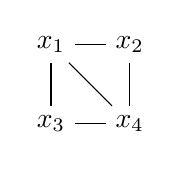
\begin{tikzpicture}
      \node (one) at (0, 1) {$x_1$};
      \node (two) at (1, 1) {$x_2$};
      \node (three) at (0, 0) {$x_3$};
      \node (four) at (1, 0) {$x_4$};
      \draw (one) -- (two);
      \draw (one) -- (three);
      \draw (one) -- (four);
      \draw (two) -- (four);
      \draw (three) -- (four);
    \end{tikzpicture}
    \caption{primal graph}
    \label{fig:primal}
  \end{subfigure}
  \begin{subfigure}[b]{0.12\textwidth}
    \centering
    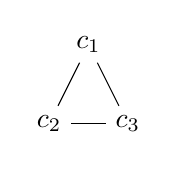
\begin{tikzpicture}
      \node (one) at (0.5, 1) {$c_1$};
      \node (two) at (0, 0) {$c_2$};
      \node (three) at (1, 0) {$c_3$};
      \draw (one) -- (two);
      \draw (one) -- (three);
      \draw (two) -- (three);
    \end{tikzpicture}
    \caption{dual graph}
    \label{fig:dual}
  \end{subfigure}
  \begin{subfigure}[b]{0.15\textwidth}
    \centering
    \begin{tikzpicture}
      \node (one) at (0.5, 1) {$c_1$};
      \node (two) at (0, 0) {$c_2$};
      \node (three) at (1, 0) {$c_3$};
      \draw (two) -- (three);
      \draw (one) -- (three);
    \end{tikzpicture}
    \caption{conflict graph}
    \label{fig:conflict}
  \end{subfigure}
  \begin{subfigure}[b]{0.17\textwidth}
    \centering
    \begin{tikzpicture}
      \node (one) at (0.5, 1) {$c_1$};
      \node (two) at (0, 0) {$c_2$};
      \node (three) at (1, 0) {$c_3$};
      \draw (one) -- (two);
    \end{tikzpicture}
    \caption{consensus graph}
    \label{fig:consensus}
  \end{subfigure}
  \begin{subfigure}[b]{0.17\textwidth}
    \centering
    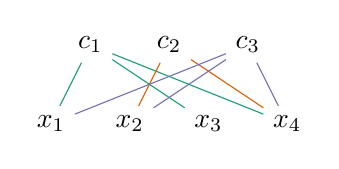
\begin{tikzpicture}
      \node (cone) at (0.5, 1) {$c_1$};
      \node (ctwo) at (1.5, 1) {$c_2$};
      \node (cthree) at (2.5, 1) {$c_3$};
      \node (xone) at (0, 0) {$x_1$};
      \node (xtwo) at (1, 0) {$x_2$};
      \node (xthree) at (2, 0) {$x_3$};
      \node (xfour) at (3, 0) {$x_4$};
      \draw[color=color1] (cone) -- (xone);
      \draw[color=color1] (cone) -- (xthree);
      \draw[color=color1] (cone) -- (xfour);
      \draw[color=color2] (ctwo) -- (xtwo);
      \draw[color=color2] (ctwo) -- (xfour);
      \draw[color=color3] (cthree) -- (xone);
      \draw[color=color3] (cthree) -- (xtwo);
      \draw[color=color3] (cthree) -- (xfour);
    \end{tikzpicture}
    \caption{incidence graph}
    \label{fig:incidence}
  \end{subfigure}
  \caption{Graphs associated with a CNF formula}
  \label{fig:graphs}
\end{figure}

\begin{figure}
  \centering
  \begin{subfigure}[b]{0.49\textwidth}
    \centering
    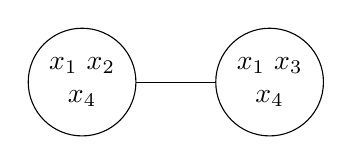
\begin{tikzpicture}[every text node part/.style={align=center}]
      \node[circle,draw] (one) {$x_1$ $x_2$\\$x_4$};
      \node[circle,draw,right=of one] (two) {$x_1$ $x_3$\\$x_4$};
      \draw (one) -- (two);
    \end{tikzpicture}
    \caption{of \cref{fig:primal}}
  \end{subfigure}
  \begin{subfigure}[b]{0.49\textwidth}
    \centering
    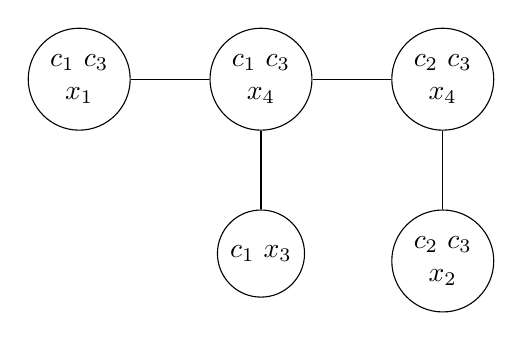
\begin{tikzpicture}[every text node part/.style={align=center}]
      \node[circle,draw] (one) {$c_1$ $c_3$\\$x_1$};
      \node[circle,draw,right=of one] (two) {$c_1$ $c_3$\\$x_4$};
      \node[circle,draw,right=of two] (three) {$c_2$ $c_3$\\$x_4$};
      \node[circle,draw,below=of two] (four) {$c_1$ $x_3$};
      \node[circle,draw,below=of three] (five) {$c_2$ $c_3$\\$x_2$};
      \draw (one) -- (two);
      \draw (two) -- (three);
      \draw (two) -- (four);
      \draw (three) -- (five);
    \end{tikzpicture}
    \caption{of \cref{fig:incidence}}
  \end{subfigure}
  \caption{Minimum-width tree decompositions (both of width two)}
  \label{fig:decompositions}
\end{figure}

Parameters for parameterized complexity results are often based on structural
properties of graphs \cite{DBLP:series/txcs/DowneyF13}, and the parameterized
complexities of $\#\SAT{}$ and \textsf{WMC} algorithms are no exception. Here we
describe several graphs derivable from a CNF formula that are used in relevant
complexity results. As an example, consider the CNF formula $(x_4 \lor \neg x_3
\lor x_1) \land (\neg x_2 \lor x_4) \land (\neg x_1 \lor x_2 \lor x_4)$. This is
a satisfiable formula with model count equal to nine. Let $c_1$, $c_2$, and
$c_3$ refer to the three clauses in the order listed. The graphs for this
formula are pictured in \cref{fig:graphs}. In both the \emph{underlying
  hypergraph} and the \emph{primal graph}\footnote{Primal graphs are known by
  many other names such as Gaifman, (variable) interaction, and variable
  incidence graphs.}, there is a node for every variable. In the former, each
clause $c$ is represented by a hyperedge that envelops the variables in $c$
whereas in the latter there is an edge between a pair of variables if they
coappear in some clause. Effectively, this means that each hyperedge of the
underlying hypergraph becomes a clique in the primal graph. Next, the
\emph{dual}, \emph{consensus}, and \emph{conflict} graphs have clauses as
variables. In the dual graph, two clauses are adjacent if they have variables in
common. In the conflict (respectively, consensus) graph, two clauses are
adjacent if they do (respectively, do not) contain complementary literals.
Finally, the \emph{incidence} graph is a bipartite graph with nodes for both
variables and clauses. An edge connects a variable $v$ to a clause $c$ if $v$
appears in $c$. Treewidth \cite{DBLP:journals/jct/RobertsonS84} and branchwidth
\cite{DBLP:journals/jct/RobertsonS91} are the two parameters used in
parameterized complexity results for $\#\SAT{}$ and \textsf{WMC}---both were
introduced by Robertson and Seymour in their seminal series of papers on graph
minors. We write \emph{primal treewidth} to refer to the treewidth of the primal
graph, and similarly for other graphs. As treewidth and tree decompositions will
be used in \cref{sec:theory}, we provide the formal definitions below and
examples of minimum-width tree decompositions of the primal and incidence graphs
of our example formula in \cref{fig:decompositions}.

\begin{definition}[\cite{DBLP:journals/jct/RobertsonS84}]
  A \emph{tree decomposition} of a graph $G$ is a pair $(T, \chi)$, where $T$ is
  a tree and $\chi\colon \mathcal{V}(T) \to 2^{\mathcal{V}(G)}$ is a labelling
  function, with the following properties:
  \begin{itemize}
  \item $\bigcup_{t \in \mathcal{V}(T)} \chi(t) = \mathcal{V}(G)$;
  \item for every edge $e \in \mathcal{E}(G)$, there exists $t \in
    \mathcal{V}(T)$ such that $e$ has both endpoints in $\chi(t)$;
  \item for all $t, t', t'' \in \mathcal{V}(T)$, if $t'$ is on the path between
    $t$ and $t''$, then $\chi(t) \cap \chi(t'') \subseteq \chi(t')$.
  \end{itemize}
  The \emph{width} of tree decomposition $(T, \chi)$ is $\max_{t \in
    \mathcal{V}(T)} |\chi(t)| - 1)$. The \emph{treewidth} of graph $G$ is the
  smallest $w$ such that $G$ has a tree decomposition of width $w$.
\end{definition}

\section{\textsf{\textmd{WMC}} Algorithms and Their Complexities}

% Mention that execution is the most computationally expensive part and this
% is the part of the algorithm that we study in \cref{sec:theory}.

Most \textsf{WMC} algorithms can be broadly classified as based on \SAT{}
solvers, knowledge compilation, or pseudo-Boolean function manipulation. Other
approaches to \textsf{WMC} not covered here include approximate
\cite{DBLP:conf/aaai/RenkensKBR14} and parallel algorithms
\cite{DBLP:conf/pgm/DalLL18,DBLP:conf/esa/FichteHWZ18}, quantum computing
\cite{DBLP:conf/ecai/Riguzzi20} and reduction to model counting
\cite{DBLP:conf/ijcai/ChakrabortyFMV15}.
\textsc{Cachet}\footnote{\url{https://cs.rochester.edu/u/kautz/Cachet/}} is a
\textsf{WMC} algorithm based on the Davis-Putnam-Logemann-Loveland (DPLL)
\cite{DBLP:journals/jacm/DavisP60,DBLP:journals/cacm/DavisLL62} search procedure
that underlies most \SAT{} algorithms, combined with component caching and
clause learning \cite{DBLP:conf/sat/SangBBKP04}.
\textsc{c2d}\footnote{\url{http://reasoning.cs.ucla.edu/c2d/}}
\cite{DBLP:conf/ecai/Darwiche04},
\textsc{d4}\footnote{\url{https://www.cril.univ-artois.fr/KC/d4.html}}
\cite{DBLP:conf/ijcai/LagniezM17}, and
\textsc{miniC2D}\footnote{\url{http://reasoning.cs.ucla.edu/minic2d/}}
\cite{DBLP:conf/ijcai/OztokD15} are all compilation algorithms that support
\textsf{WMC}. \textsc{c2d} compiles to deterministic decomposable negation
normal form (d-DNNF) \cite{DBLP:journals/jancl/Darwiche01}. Similarly,
\textsc{d4} compiles to decision-DNNF (also known as decomposable decision
graphs) \cite{DBLP:conf/aaai/FargierM06}. The only difference between d-DNNF and
decision-DNNF is that decision-DNNF has if-then-else constructions instead of
disjunctions \cite{DBLP:conf/ijcai/LagniezM17}. With both \textsc{c2d} and
\textsc{d4}, we use
\textsc{query-dnnf}\footnote{\url{http://www.cril.univ-artois.fr/kc/d-DNNF-reasoner.html}}
to compute the numerical answer from the compiled circuit. Finally,
\textsc{miniC2D} \cite{DBLP:conf/ijcai/OztokD15} compiles to decision-SDDs---a
subset of sentential decision diagrams (SDDs) that form a subset of d-DNNF
\cite{DBLP:conf/ijcai/Darwiche11}.

All of the algorithms mentioned above are $\#\SAT{}$ algorithms that were later
adapted to support weights. Two recently proposed \textsf{WMC} algorithms
instead use data structures that natively support weights and can thus take
advantage of redundancies in the numerical values of weights or other numbers.
These data structures are representations of \emph{pseudo-Boolean functions},
i.e., functions of the form $2^X \to \mathbb{R}$, where $X$ is a set, and $2^X$
denotes its powerset. \textsc{ADDMC} is the first such algorithm
\cite{DBLP:conf/aaai/DudekPV20}. It uses \emph{algebraic decision diagrams}
(ADDs) \cite{DBLP:journals/fmsd/BaharFGHMPS97} as the representation for
pseudo-Boolean functions (ADDs are described in more detail in \cref{sec:adds}).
\textsc{DPMC}\footnote{\url{https://github.com/vardigroup/dpmc}} extends
\textsc{ADDMC} in two ways \cite{DBLP:conf/cp/DudekPV20}. First, \textsc{DPMC}
allows for the order and nesting of operations on ADDs to be determined from an
approximately-minimal-width tree decomposition rather than by heuristics.
Second, tensors are offered as an alternative to ADDs. In this paper, we focus
on tree decomposition-based planning and ADD-based execution---the
best-performing combination in the original set of experiments
\cite{DBLP:conf/cp/DudekPV20}. Note that the complexity results in
\cref{sec:theory} apply equally to both \textsc{ADDMC} and \textsc{DPMC} (with
the observation that the implicit tree decomposition used by \textsc{ADDMC} may
have significantly higher width), but we omit \textsc{ADDMC} from our
experiments in \cref{sec:experiments} because it would exceed time and memory
limits on too many instances.

Some parameterized complexity results already exist for \textsc{Cachet}
\cite{DBLP:conf/sat/SangBBKP04} and \textsc{c2d}
\cite{DBLP:conf/ecai/Darwiche04} but not for \textsc{d4}
\cite{DBLP:conf/ijcai/LagniezM17} or \textsc{miniC2D}
\cite{DBLP:conf/ijcai/OztokD15} (and the complexity of \textsc{ADDMC}
\cite{DBLP:conf/aaai/DudekPV20} and \textsc{DPMC} \cite{DBLP:conf/cp/DudekPV20}
is the topic of \cref{sec:theory}). While the complexity of \textsc{Cachet} has
not been analysed directly, \textsc{Cachet} is based on component caching which
is known to have a $2^{\mathcal{O}(w)}n^{\mathcal{O}(1)}$ time complexity (where
$n$ is the number of variables, and $w$ is the branchwidth of the underlying
hypergraph) \cite{DBLP:journals/jair/BacchusDP09,DBLP:conf/sat/SangBBKP04}.
Interestingly, \textsc{c2d} is specifically designed to handle high primal
treewidth (which the author calls \emph{connectivity}
\cite{DBLP:conf/ijcai/Darwiche99}) and improves upon an earlier algorithm that
has $\mathcal{O}(mw2^w)$ time complexity (where $m$ is the number of clauses,
and $w$ is the width of the decomposition tree which is known to be at most
primal treewidth)
\cite{DBLP:journals/jacm/Darwiche01,DBLP:conf/ecai/Darwiche04}.

Parameterized complexity of $\#\SAT{}$ is a much more studied subject.
$\#\SAT{}$ is known to be \emph{fixed-parameter tractable} (\FPT{}; i.e., the
problem can be solved in $f(k)\lVert\phi\rVert^{\mathcal{O}(1)}$ time, where $f$
is some computable function, and $\lVert\phi\rVert$ is the length of the
formula) with respect to (w.r.t.) incidence treewidth as a consequence of
Courcelle's Theorem (i.e., model count is definable in monadic second-order
logic) \cite{DBLP:journals/dam/CourcelleMR01}. Parameters that are known to make
$\#\SAT{}$ \FPT{} include primal, dual, and incidence treewidth
\cite{DBLP:journals/jda/SamerS10}. Ganian and Szeider
\cite{DBLP:journals/ai/GanianS21} also show $\#\SAT{}$ to be \FPT{} w.r.t.
consensus treewidth and \W{}[1]-hard (i.e., not \FPT{} under standard
assumptions) w.r.t. conflict treewidth. They also introduce another parameter
that makes $\#\SAT{}$ \FPT{}, which is inspired by modularity of graphs.

\todo[inline]{TODO: reference and describe modularity.}

\section{Parameterized Complexity of \textsc{DPMC}} \label{sec:theory}

For any graph $G$, we write $\mathcal{V}(G)$ for its set of vertices,
$\mathcal{E}(G)$ for its set of edges. If $G$ is a tree (respectively, a
directed graph), then we denote its set of leaves (respectively, sinks) as
$\mathcal{L}(G)$, and $\mathcal{C}(v)$ denotes the children (respectively,
direct successors) of a vertex $v \in \mathcal{V}(G)$. For any function $f\colon
X \to Y$, we denote its domain as $\dom(f)$ (i.e., $\dom(f) = X$) and its
codomain as $\cod(f)$ (i.e., $\cod(f) = Y$). We write $\mathbb{N}_0$ and
$\mathbb{N}^+$ for natural numbers with and without zero, respectively.

We generalise some notation for pseudo-Boolean functions from previous work
\cite{my_sat_paper}. Let $X$ be a set of variables, $\phi$ a propositional
formula over $X$, and $f, g\colon 2^X \to \mathbb{R}$ pseudo-Boolean functions.
We write $[\phi]_g^f$ to denote a function $2^X \to \mathbb{R}$ defined as
\[
  [\phi]^f_g(Y) \coloneqq
  \begin{cases}
    f(Y) & \text{if } Y \models \phi \\
    g(Y) & \text{if } Y \not\models \phi
  \end{cases}
\]
for any $Y \subseteq X$. Two special cases will be particularly useful. First,
if $f$ and $g$ are real numbers instead, they are to be interpreted as constant
pseudo-Boolean functions $2^X \to \mathbb{R}$. Second, if $\phi$ is just a
variable name, then $Y \models \phi$ is equivalent to $\phi \in Y$.

\subsection{ADDs, Operations on ADDs, and Their Complexities} \label{sec:adds}

Our definition of an ADD is partially based on the original definition
\cite{DBLP:journals/fmsd/BaharFGHMPS97} as well as more recent work
\cite{DBLP:conf/cp/DudekPV20} but states some details more explicitly. The
definition can also be stated more generally to use any set instead of
$\mathbb{R}$ and include the possibility of a single ADD representing multiple
functions.

\begin{definition}
  Given a set of variables $X$ and a variable ordering represented as an injection
  $\sigma\colon X \to \mathbb{N}^+$, an \emph{ADD} is a tuple $(G, r, \rho,
  \chi, \epsilon)$ where:
  \begin{itemize}
  \item $G$ is a rooted directed acyclic graph with root $r \in \mathcal{V}(G)$
    (i.e., there is a directed path from $r$ to any other node),
  \item $\rho\colon \mathcal{L}(G) \to \mathbb{R}$ labels sinks with real
    numbers,
  \item $\chi\colon \mathcal{V}(G) \setminus \mathcal{L}(G) \to X$ labels other
    nodes with variable names,
  \item and $\epsilon\colon \mathcal{E}(G) \to \{\,0, 1\,\}$ labels edges.
  \end{itemize}
  Moreover, the following properties must be satisfied.
  \begin{itemize}
  \item Every node has outdegree either zero or two. In the latter case, the two
    outgoing edges $e, f \in \mathcal{E}(G)$ are such that $\epsilon(e) = 1$,
    and $\epsilon(f) = 0$. If $e = (v, u)$, and $f = (v, w)$ for some $u, v, w
    \in \mathcal{V}(G)$, then $u$ is the \emph{positive successor} of $v$, and
    $w$ is the \emph{negative successor}.
  \item For every directed path with node sequence $v_1, v_2, \dots, v_n$ such
    that $v_i \not\in \mathcal{L}(G)$ for all $i$, we have that
    $\sigma(\chi(v_i)) < \sigma(\chi(v_{i+1}))$ for all $i = 1, 2, \dots, n -
    1$.
  \end{itemize}
  We say that an ADD \emph{has} variable $x \in X$ if there is a node $v \in
  \mathcal{V}(G) \setminus \mathcal{L}(G)$ such that $\chi(v) = x$.

  It remains to define how an ADD can be interpreted as a pseudo-Boolean
  function. Let $\llbracket \cdot \rrbracket\colon \mathcal{V}(G) \to
  \mathbb{R}^{2^X}$ be defined as
  \[
    \llbracket v \rrbracket \coloneqq
    \begin{cases}
      \rho(v) & \text{if } v \in \mathcal{L}(G) \\
      [\chi(v)]^{\llbracket u \rrbracket}_{\llbracket w \rrbracket} &
      \text{if } v \not\in \mathcal{L}(G)
    \end{cases}
  \]
  for all $v \in \mathcal{V}(G)$, where $u \in \mathcal{V}(G)$ and $w \in
  \mathcal{V}(G)$ are the positive and negative successors of $v$, respectively.
  Here, $\llbracket \cdot \rrbracket$ returns a pseudo-Boolean function $2^X \to
  \mathbb{R}$ for each node of $G$, and the interpretation of the ADD itself is
  defined to be $\llbracket r \rrbracket$. As before, $\rho(v)$ should be
  interpreted as a constant function.
\end{definition}

\begin{fact}[\cite{DBLP:journals/fmsd/BaharFGHMPS97}]
  For any fixed set of variables $X$ and ordering function $\sigma\colon X \to
  \mathbb{N}^+$, there is a unique (up to isomorphism) \emph{canonical} ADD for
  every pseudo-Boolean function $2^Y \to S$ for all $Y \subseteq X$. Any ADD can
  be \emph{reduced} to its canonical form in time linear in the number of nodes.
\end{fact}

\begin{figure}
  \centering
  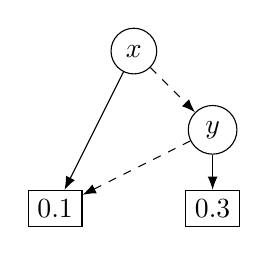
\begin{tikzpicture}
    \node[circle,draw] (x) at (0, 0) {$x$};
    \node[circle,draw] (y) at (1, -1) {$y$};
    \node[draw] (a) at (-1, -2) {0.1};
    \node[draw] (b) at (1, -2) {0.3};
    \draw[-Latex,dashed] (x) -- (y);
    \draw[-Latex] (x) -- (a);
    \draw[-Latex,dashed] (y) -- (a);
    \draw[-Latex] (y) -- (b);
  \end{tikzpicture}
  \label{fig:add}
  \caption{A graphical representation of the ADD from \cref{example:add}. Sinks
    are represented as rectangles and other nodes as circles. The labels of
    nodes are written directly on them. An edge $e$ is dashed if $\epsilon(e) =
    0$ and solid otherwise.}
\end{figure}

\begin{example} \label{example:add}
  Let $f\colon 2^{\{\,x, y\,\}} \to \mathbb{R}$ be a pseudo-Boolean function
  defined as $f(\emptyset) = f(\{\,x\,\}) = f(\{\,x, y\,\}) = 0.1$, and
  $f(\{\,y\,\}) = 0.3$ and $\sigma\colon \{\,x, y\,\} \to \mathbb{N}^+$ be
  the variable ordering function defined as $\sigma(x) = 1$, and $\sigma(y) =
  2$. Then the canonical ADD for $f$ under $\sigma$ is pictured in
  \cref{fig:add} and can be formally defined as $(G, a, \rho, \chi, \epsilon)$,
  where:
  \begin{itemize}
  \item $\mathcal{V}(G) = \{\,a, b, c, d\,\}$,
  \item $\mathcal{E}(G) = \{\,(a, b), (a, c), (b, c), (b, d)\,\}$,
  \item $\rho(c) = 0.1$, $\rho(d) = 0.3$,
  \item $\chi(a) = x$, $\chi(b) = y$,
  \item $\epsilon((a, c)) = \epsilon((b, d)) = 1$, $\epsilon((a, b)) =
    \epsilon((b, c)) = 0$.
  \end{itemize}
\end{example}

\begin{table}
  \centering
  \caption{Operations on ADDs, their definitions, the time complexity of the
    best-known algorithm for performing each operation, and references to the
    papers that introduced these algorithms. Let $f\colon 2^X \to \mathbb{R}$
    and $g\colon 2^Y \to \mathbb{R}$ be pseudo-Boolean functions represented by
    ADDs with $n$ and $m$ nodes respectively, and let $r \in \mathbb{R}$, and $x
    \in X$.}
  \label{tbl:complexity}
  \begin{tabular}{llll}
    \toprule
    Operation & Definition & Complexity & Source \\
    \midrule
    reduce $f$ & & $\mathcal{O}(n)$ & \cite{somenzi1998cudd} \\
    $r+f$, $rf$ & $r+f\colon 2^X \to \mathbb{R}$, $(r+f)(Z) \coloneqq r+f(Z)$ & $\mathcal{O}(n)$ & \cite{DBLP:journals/tc/Bryant86} \\
    $f+g$, $fg$ & $f+g\colon 2^{X \cup Y} \to \mathbb{R}$, $(f+g)(Z) \coloneqq f(Z)+g(Z)$ & $\mathcal{O}(mn)$ & \cite{DBLP:journals/tc/Bryant86} \\
    $f|_{x=0}$ & $f|_{x=0}\colon 2^{X \setminus \{\,x\,\}} \to \mathbb{R}$, $f|_{x=0}(Z) \coloneqq f(Z)$ & $\mathcal{O}(n)$ & \cite{DBLP:journals/tc/Bryant86} \\
    $f|_{x=1}$ & $f|_{x=1}\colon 2^X \to \mathbb{R}$, $f|_{x=1}(Z) \coloneqq f(Z \cup \{\,x\,\})$ & $\mathcal{O}(n)$ & \cite{DBLP:journals/tc/Bryant86} \\
    $\exists_xf$ & $\exists_xf\colon 2^{X \setminus \{\,x\,\}} \to \mathbb{R}$, $\exists_xf(Z) \coloneqq f|_{x=0}(Z) + f|_{x=1}(Z)$ & $\mathcal{O}(n^2)$ & a corollary of other results \\
    \bottomrule
  \end{tabular}
\end{table}

Various operations can be defined on ADDs. We list the ones pertinent to our
needs in \cref{tbl:complexity}: reduction of an ADD to its canonical form,
addition/multiplication as well as scalar addition/multiplication, two types of
\emph{restrictions}, and \emph{projection}. For a more detailed description, we
refer the reader to previous work
\cite{DBLP:journals/fmsd/BaharFGHMPS97,my_uai_paper,DBLP:conf/aaai/DudekPV20}.
Throughout the paper, we assume that projection has the lowest precedence and
extend the definition to allow for sets of variables. For any $W = \{\,w_1, w_2,
\dots, w_k\,\} \subseteq X$, let $\exists_W f\colon 2^{X \setminus W} \to
\mathbb{R}$ be defined as $\exists_Wf(Z) \coloneqq
\exists_{w_1}\exists_{w_2}\cdots\exists_{w_k}f(Z)$ for all $Z \subseteq X
\setminus W$, where the order of $w_i$'s is immaterial. We assume that after
every operation on ADDs, the resulting ADD is reduced to its canonical form and
write `the ADD for some function' to mean `the \emph{canonical} ADD'. In line
with \textsc{DPMC} \cite{DBLP:conf/cp/DudekPV20}, we consider $X$ and $\sigma$
to be fixed throughout the execution of the algorithm, with $X$ containing all
relevant variables.

\begin{fact} \label{lemma:add_size}
  The ADD for a pseudo-Boolean function $2^X \to \mathbb{R}$ has at most
  $2^{|X|+1}$ nodes. This upper bound is achieved when the function is
  injective.
\end{fact}

\begin{lemma} \label{lemma:clause_time}
  Let $\phi$ be a conjunction/disjunction of $n$ literals. Then the ADD for
  $[\phi]^p_q$ (for any $p, q \in \mathbb{R}$ such that $p \ne q$) can be
  constructed in $\mathcal{O}(2^n)$ time.
\end{lemma}
\begin{proof}
  The ADD for $[\phi]_0^1$ can be constructed with a sequence of $n-1$ binary
  operations, with one of the two operands always the ADD representation of a
  literal. The number of variables in the other operand then follows the
  sequence $1, 2, 3, \dots, n-1$. By \cref{lemma:add_size}, the numbers of nodes
  in the ADDs for these operands is then $2^2, 2^3,
  \dots, 2^n$. Since one of the operands is of constant size,
  the overall time complexity of all binary operations is then
  $\sum_{i=2}^n \mathcal{O}(2^i) = \mathcal{O}(2^n)$. Finally, note that
  $[\phi]_q^p = (p-q)[\phi]_0^1 + q$. As scalar operations can be performed in
  linear time, the overall complexity remains $\mathcal{O}(2^n)$.
\end{proof}

\subsection{Main Result}

We begin by compiling relevant results from previous work with some slight
modifications.

\begin{definition}[\cite{DBLP:conf/cp/DudekPV20}]
  Let $X$ be a set of variables and $\phi$ be a CNF formula over $X$. A
  \emph{project-join tree} (PJT) of $\phi$ is a tuple $(T, r, \gamma, \pi)$
  where:
  \begin{itemize}
  \item $T$ is a tree with root $r \in \mathcal{V}(T)$,
  \item $\gamma\colon \mathcal{L}(T) \to \phi$ is a bijection between the leaves of
    $T$ and the clauses of $\phi$, and
  \item $\pi\colon \mathcal{V}(T) \setminus \mathcal{L}(T) \to 2^X$ is a
    labelling function on internal nodes.
  \end{itemize}
  Moreover, the following properties must be satisfied.
  \begin{itemize}
  \item $\{\,\pi(t) : t \in \mathcal{V}(T) \setminus \mathcal{L}(T)\,\}$ is a
    partition of $X$, and
  \item for each internal node $t \in \mathcal{V}(T) \setminus \mathcal{L}(T)$,
    variable $x \in \pi(t)$, and clause $c \in \phi$ such that $x$ appears in
    $c$, the leaf node $\gamma^{-1}(c)$ must be a descendant of $t$ in $T$.
  \end{itemize}
\end{definition}

Let $(T, r, \gamma, \pi)$ be a PJT. We can encapsulate the operations on ADDs
performed during \textsc{DPMC} \cite{DBLP:conf/cp/DudekPV20} execution by
$\delta(r)$, where $\delta\colon \mathcal{V}(T) \to \mathbb{R}^{\cod(\pi)}$ is a
recursive function defined as
\begin{equation} \label{eq:execution}
  \delta(t) \coloneqq
  \begin{cases}
    \gamma(t) & \text{if } t \in \mathcal{L}(T) \\
    \exists_{\pi(t)} \prod_{u \in \mathcal{C}(t)} \delta(u) \prod_{x \in \pi(t)} [x]_{w(\neg x)}^{w(x)} & \text{if } t \not\in \mathcal{L}(T) \text{.\footnotemark}
  \end{cases}
\end{equation} \footnotetext{This is a variation of Eq. (2) in the \textsc{DPMC}
  paper \cite{DBLP:conf/cp/DudekPV20}.}
The range of $\delta(r)$ then contains a single real number, i.e., the answer.

\begin{definition}[The Width of a PJT
  \cite{DBLP:conf/cp/DudekPV20}] \label{def:size}
  Let $(T, r, \gamma, \pi)$ be a PJT and $\mathtt{Vars}\colon \mathcal{V}(T) \to
  \cod(\pi)$ and $\mathtt{size}\colon \mathcal{V}(T) \to \mathbb{N}_0$ be two
  functions defined on the nodes of the PJT defined respectively as
  \[
    \mathtt{Vars}(t) \coloneqq
    \begin{cases}
      X & \text{if } t \in \mathcal{L}(T) \text{ and } \dom(\gamma(t)) = 2^X
      \\
      \left( \bigcup_{u \in \mathcal{C}(t)} \mathtt{Vars}(u) \right) \setminus
      \pi(t) & \text{if } t \not\in \mathcal{L}(T)
    \end{cases}
  \]
  and
  \[
    \mathtt{size}(t) \coloneqq
    \begin{cases}
      |\mathtt{Vars}(t)| & \text{if } t \in \mathcal{L}(T) \\
      |\mathtt{Vars}(t) \cup \pi(t)| & \text{if } t \not\in \mathcal{L}(T)
    \end{cases}
  \]
  for any $t \in \mathcal{V}(T)$. Intuitively, $\mathtt{size}(t)$ is the maximum
  number of variables that can appear during the computation of $\delta(t)$
  (excluding recursive calls). The \emph{width} of a PJT $(T, r, \gamma, \pi)$
  is then $\max_{t \in \mathcal{V}(T)} \mathtt{size}(t)$.
\end{definition}

We are now ready to state the parameterized complexity of \textsc{DPMC}
\cite{DBLP:conf/cp/DudekPV20}.

\begin{theorem} \label{thm:main}
  Let $\phi$ be a CNF formula over a set of variables $X$ and $(T, r, \gamma,
  \pi)$ be its PJT of width $w$. Then \textsc{DPMC}
  \cite{DBLP:conf/cp/DudekPV20} runs in time $\mathcal{O}(4^wmn)$, where $m =
  |\mathcal{L}(T)| = |\phi|$ is the number of clauses, and $n = |X|$ is the
  number of variables.
\end{theorem}
\begin{proof}
  We consider the complexity of constructing ADD representations of the clauses
  in $\phi$ and the complexity of multiplication and projection operations
  throughout the recursive calls of $\delta$ from \cref{eq:execution}. Let $t
  \in \mathcal{L}(T)$ be a leaf. Note that $\mathtt{size}(t) \le w$ by
  \cref{def:size}. Assuming that clauses have no repeating variables, it takes
  $\mathcal{O}(2^w)$ time to construct $\delta(t)$ by \cref{lemma:clause_time}
  and $\mathcal{O}(2^wm)$ time to construct all leaves of the PJT.

  Now let $t \in \mathcal{V}(T) \setminus \mathcal{L}(T)$ be an internal node.
  Here we multiply $|\mathcal{C}(t)|$ ADDs from recursive calls with $|\pi(t)|$
  constant-sized ADDs that hold the relevant weights and project the variables
  in $\pi(t)$. We assume that $\prod_{u \in \mathcal{C}(t)} \delta(u)$ is
  computed first, and then multiplied by each $[x]_{w(\neg x)}^{w(x)}$ for all
  $x \in \pi(t)$. Note that $|\mathcal{C}(t)| \le |\mathcal{L}(T)| = m$,
  $|\pi(t)| \le w$, and the ADDs involved can have up to $w$ variables. This
  means that each ADD has $\mathcal{O}(2^w)$ nodes regardless of whether it
  comes from $\mathcal{C}(t)$ or from multiplications.

  Each multiplication of ADDs from recursive calls takes $\mathcal{O}(4^w)$ time
  by \cref{tbl:complexity}, and so all such multiplications will take
  $\mathcal{O}(4^wm)$ time for $t$ and $\mathcal{O}(4^wmn)$ time across all $t
  \in \mathcal{V}(T) \setminus \mathcal{L}(T)$ since the number of internal
  nodes in the PJT is bounded by the number of variables.

  Each multiplication of a constant-sized ADD and an ADD with $\mathcal{O}(2^w)$
  nodes will take $\mathcal{O}(2^w)$ time, and so $|\pi(t)|$ of them will take
  $\mathcal{O}(2^ww)$ time. Summing this across all internal nodes of the PJT
  gives $\mathcal{O}(2^wwn)$.

  Each variable is projected exactly once and is always projected from an ADD
  with at most $\mathcal{O}(2^w)$ nodes. Thus, the time complexity of projecting
  all variables is $\mathcal{O}(4^wn)$. Overall, we get $\mathcal{O}(2^wm)$ time
  for constructing initial ADDs, $\mathcal{O}(4^wmn)$ and $\mathcal{O}(2^wwn)$
  for the two types of multiplications, and $\mathcal{O}(4^wn)$ for projections,
  resulting in $\mathcal{O}(4^wmn)$ time in total.
\end{proof}

The PJT of a formula is (efficiently) constructed from an
approximately-minimal-width tree decomposition of its primal graph. Moreover,
Dudek et al. \cite{DBLP:conf/cp/DudekPV20} show that if the tree decomposition
has width $w$, then the PJT will have width at most $w+1$. This allows us to
restate \cref{thm:main} without referring to PJTs.

\begin{corollary}
  Given a \textsf{WMC} instance with a CNF formula $\phi$ with a tree
  decomposition of its primal graph of width $w$, \textsc{DPMC}
  \cite{DBLP:conf/cp/DudekPV20} runs in time $\mathcal{O}(4^wmn)$, where $m$ is
  the number of clauses, and $n$ is the number of variables.
\end{corollary}

Since the $4^w$ part is tight (because the multiplication of two ADDs with $m$
and $n$ nodes is $\Theta(mn)$ when the corresponding pseudo-Boolean functions
are injective, and all possible products of their values are different), we can
conjecture that \textsc{DPMC} \cite{DBLP:conf/cp/DudekPV20} performs worse
on high-primal-treewidth instances compared to other algorithms such as
\textsc{c2d} \cite{DBLP:conf/ecai/Darwiche04} which scales at most as $2^w$
w.r.t. primal treewidth. \cref{sec:experiments} tests this conjecture on
randomly generated \textsf{WMC} instances.

\section{Random $k$-CNF Formulas with Varying Primal Treewidth}

% For instance, if a variable $x$ with $w(x) = w(\neg x) = 1$ does not appear in
% the formula, \textsc{Cachet} \cite{DBLP:conf/sat/SangBBKP04} divides the
% answer by two whereas other algorithms do not.

Let $S$ be a finite set. We write $\mathcal{U}S$ for the discrete uniform
probability distribution on $S$. We represent any other probability distribution
as a pair $(S, p)$ where $p\colon S \to [0, 1]$ is a probability mass function.
For any probability distribution $\mathcal{P}$, we write $x \leftlsquigarrow
\mathcal{P}$ to denote the act of sampling $x$ from $\mathcal{P}$.

Our random $k$-CNF model is based on the following parameters:
\begin{itemize}
\item the number of variables $\nu \in \mathbb{N}^+$,
\item (clause) \emph{density} $\mu \in \mathbb{R}_{>0}$ (i.e., the ratio of
  the number of clauses and the number of variables),
\item clause width $\kappa \in \mathbb{N}^+$ (for $k$-CNF formulas, $\kappa =
  k$),
\item a parameter $\rho \in [0, 1]$ that influences the primal treewidth of
  the formula,
\item the proportion $\delta \in [0, 1]$ of variables $x$ such that $w(x) = 1$
  and $w(\neg x) = 0$ or $w(x) = 0$ and $w(\neg x) = 1$,
\item and the proportion $\epsilon \in [0, 1-\delta]$ of variables $x$ such that
  $w(x) = w(\neg x) = 0.5$.
\end{itemize}

\begin{remark}
  Note that not having a parameter that in some way influences primal treewidth
  is unrealistic for generating instances with a wide range of primal treewidth
  values. Without such a parameter (i.e., if $\rho=0$), the variance of primal
  treewidth is relatively small compared to the range of values one could
  generate by varying $\rho$ between zero and one (evidence for this is
  presented in \cref{sec:remarks}).
\end{remark}

\begin{remark}
  The parameters $\delta$ and $\epsilon$ that control the numerical values of
  weights are part of the model because the running time of \textsc{DPMC}
  \cite{DBLP:conf/cp/DudekPV20} (and other algorithms based on ADDs) depends on
  these numerical values. Indeed, the running time depends on the numbers of
  nodes in various ADDs, and this depends on the range of each pseudo-Boolean
  function. If all weights are different real numbers in $(0, 1)$, then
  performing addition and multiplication on them is unlikely to result in any
  duplicates, and the numbers of nodes in ADDs is maximised. But weights such as
  zero and one are particularly `simplifying' because they are respectively the
  additive and multiplicative identities. Including many copies of the same
  weight (such as 0.5) can be somewhat simplifying as well.
\end{remark}

\begin{algorithm}
  \caption{Generating a random $k$-CNF formula}
  \label{alg:random}
  \SetKwData{kcnf}{kcnf}
  \SetKwFunction{NewVariable}{NewVariable}
  \SetKwProg{Fn}{Function}{:}{}
  \KwData{$\nu,\kappa \in \mathbb{N}^+$ such that $\kappa < \nu$, $\mu \in
    \mathbb{R}_{>0}$, $\rho \in [0, 1]$.}
  \KwResult{A $k$-CNF formula $\phi$.}
  $\phi \gets \text{empty CNF formula}$\;
  $G \gets \text{empty graph}$\;
  \For{$i \gets 1$ \KwTo $\lfloor \nu\mu \rfloor$}{
    $X \gets \emptyset$\;
    \For{$j \gets 1$ \KwTo $\kappa$}{
      $x \gets \NewVariable{$X$, $G$}$\;
      $\mathcal{V}(G) \gets \mathcal{V}(G) \cup \{\, x \,\}$\; \label{line:7}
      $\mathcal{E}(G) \gets \mathcal{E}(G) \cup \{\, \{\,x, y\,\} \mid y \in X
      \,\}$\; \label{line:8}
      $X \gets X \cup \{\, x \,\}$\; \label{line:9}
    }
    $\phi \gets \phi \cup \{\, l \leftlsquigarrow \mathcal{U}\{\, x, \neg x \,\}
    \mid x \in X \,\}$\; \label{line:construct_clause}
  }
  \Return{$\phi$}\;
  \Fn{\NewVariable{$X$, $G$}}{
    $N \gets \{\, e \in \mathcal{E}(G) \mid |e \cap X| = 1
    \,\}$\; \label{line:13}
    \lIf{$N = \emptyset$}{\Return{$x \leftlsquigarrow \mathcal{U}(\{\, x_1, x_2,
        \dots, x_\nu \,\} \setminus X)$}}
    \Return{$x \leftlsquigarrow \left(\{\, x_1, x_2, \dots, x_\nu \,\} \setminus
        X, y \mapsto \frac{1 - \rho}{\nu - |X|} + \rho\frac{|\{\, z \in X \mid
          \{\,y, z\,\} \in \mathcal{E}(G)
          \,\}|}{|N|}\right)$}\; \label{line:return}
  }
\end{algorithm}

The process behind generating random $k$-CNF formulas is summarised as
\cref{alg:random}. For the rest of this section, let $x_1, x_2, \dots, x_\nu$ be
the variables of the formula that is being generated. We simultaneously
constructs both formula $\phi$ and its primal graph $G$. Each execution of the
first for-loop adds a clause to $\phi$. This is done by constructing a set $X$
of variables to be included in the clause, and then randomly adding either $x$
or $\neg x$ to the clause for each $x \in X$ on \cref{line:construct_clause}.
Function \texttt{NewVariable} randomly selects each new variable $x$, and
\cref{line:7,line:8,line:9} add $x$ to the graph and the formula while also
adding edges between $x$ and all the other variables in the clause. To select
each variable, \cref{line:13} defines set $N$ to contain all edges with exactly
one endpoint in $X$. The edges that will be added to $G$ by \cref{line:8} will
form a subset of $N$. If $N$ is empty, we select the variable uniformly at
random (u.a.r.) from all viable candidates. Otherwise, $\rho$ determines how
much we bias the uniform distribution towards variables that would introduce the
smallest number of new edges to $G$. Note that when $\rho=0$, \cref{alg:random}
reduces to the standard random model for $k$-CNF formulas where each clause has
no duplicate variables. Also note that on \cref{line:return} the probability
that a variable is selected to be included in a clause scales linearly w.r.t.
the proportion of edges in $N$ that would be repeatedly added to $G$ if the
variable $y$ was added to the clause. This is an arbitrary choice (which appears
to work well, see \cref{exp:regular_satisfiability} and
\cref{fig:regular_repetitiveness}) although alternatives (e.g., exponential
scaling) could be considered.

To transform the generated $k$-CNF formula into a \textsf{WMC} instance, we need
to define weights on literals.\footnote{Note that algorithms such as
  \textsc{DPMC} \cite{DBLP:conf/cp/DudekPV20} and \textsc{ADDMC}
  \cite{DBLP:conf/aaai/DudekPV20} support a more flexible way of assigning
  weights that can lead to significant performance improvements
  \cite{my_uai_paper,my_sat_paper}.} We want to partition all variables into
three groups: those with weights equal to zero and one, those with weights equal
to 0.5, and those with arbitrary weights, where the size of each group is
determined by $\delta$ and $\epsilon$. To do this, we sample a permutation $\pi
\leftlsquigarrow \mathcal{U}S_\nu$ (where $S_\nu$ is the permutation group on $\{
1, 2, \dots, \nu \}$), and assign to each \emph{variable} $x_n$ a weight drawn
u.a.r. from
\begin{itemize}
\item $\mathcal{U}\{\,0, 1\,\}$ if $\pi(n) \le \nu\delta$,
\item $\mathcal{U}\{\,0.5\,\}$ if $\nu\delta < \pi(n) \le \nu\delta +
  \nu\epsilon$,
\item and $\mathcal{U}\{\, 0.01, 0.02, \dots, 0.99 \,\}$\footnote{The interval
    $(0, 1)$ is represented as 99 discrete values purely for convenience.} if
  $\pi(n) > \nu\delta + \nu\epsilon$.
\end{itemize}
We extend these weights to weights on \emph{literals} by choosing the weight of
each positive literal to be equal to the weight of its variable, and the weight
of each negative literal to be such that $w(x) + w(\neg x) = 1$ for all
variables $x$. This restriction is to ensure consistent answers among the
algorithms.

\begin{example} \label{example:algorithm}
  Let $\nu = 5$, $\mu = 0.6$, $\kappa = 3$, $\rho = 0.3$, $\delta = 0.4$,
  and $\epsilon = 0.2$ and consider how \cref{alg:random} generates a random
  instance. Since $\kappa = 3$, and $\lfloor\nu\mu\rfloor = 3$,
  \cref{alg:random} will generate a 3-CNF formula with three clauses.

  For the first variable of the first clause, we are choosing u.a.r. from $\{\,
  x_1, x_2, \dots, x_5 \,\}$. Suppose the algorithm chooses $x_5$. The graph $G$
  then gets its first node but no edges. The second variable is chosen u.a.r.
  from $\{\, x_1, x_2, x_3, x_4 \,\}$. Suppose the second variable is $x_2$.
  Then $G$ gets another node and its first edge between $x_2$ and $x_5$. The
  third variable in the first clause is similarly chosen u.a.r. from $\{\, x_1,
  x_3, x_4 \,\}$ because the only edge in $G$ has both endpoints in $X = \{\,
  x_2, x_5 \,\}$, and so $N = \emptyset$. Suppose the third variable is $x_1$.
  The graph $G$ becomes a triangle connecting $x_1$, $x_2$, and $x_5$. Each of
  the three variables is then added to the clause as either a positive or a
  negative literal (with equal probabilities). Thus, the first clause becomes,
  e.g., $\neg x_5 \lor x_2 \lor x_1$.

  The first variable of the second clause is chosen u.a.r. from $\{\, x_1, x_2,
  \dots, x_5\,\}$.\footnote{Note that the first variable of any clause is always
    chosen this way.} Suppose it is $x_5$ again. When the function
  \texttt{NewVariable} tries to choose the second variable, $X = \{\, x_5 \,\}$,
  and so $N = \{\, \{\, x_1, x_5 \,\}, \{\, x_2, x_5 \,\}\,\}$. The second
  variable is chosen from the discrete probability distribution
  \[
    \Pr(x_1) = \Pr(x_2) = \frac{1 - 0.3}{5 - 1} + 0.3 \times \frac{1}{2} = 0.325
  \]
  and
  \[
    \Pr(x_3) = \Pr(x_4) = \frac{1 - 0.3}{5 - 1} = 0.175.
  \]

  We skip the details of how all remaining variables and clauses are selected
  and consider the weight assignment. First, we shuffle the list of variables
  and get, e.g., $L = (x_4, x_3, x_2, x_1, x_5)$, i.e., the permutation $\pi$ is
  \[
    \pi =
    \begin{pmatrix}
      1 & 2 & 3 & 4 & 5\\
      4 & 3 & 2 & 1 & 5
    \end{pmatrix}
  \]
  which means that the first $\nu\delta = 5 \times 0.4 = 2$ variables of $L$ get
  weights u.a.r. from $\{\, 0, 1 \,\}$, the next $\nu\epsilon = 5 \times 0.2 =
  1$ variable gets $0.5$ weight, and the remaining two variables get weights
  u.a.r. from $\{\,0.01, 0.02, \dots, 0.99 \,\}$. The weight function $w\colon
  \{\, x_1, x_2, \dots, x_5, \neg x_1, \neg x_2, \dots, \neg x_5\,\} \to [0, 1]$
  can then be defined as, e.g., $w(x_4) = w(\neg x_3) = 0$, $w(x_3) = w(\neg
  x_4) = 1$, $w(x_2) = w(\neg x_2) = 0.5$, $w(x_1) = 0.23$, $w(\neg x_1) =
  0.77$, $w(x_5) = 0.18$, and $w(\neg x_5) = 0.82$.
\end{example}

\subsection{Validating the Model} \label{sec:remarks}

In this section, we briefly discuss the following two questions.
\begin{itemize}
\item Are instances generated with higher values of $\rho$ less likely to be
  satisfiable?
\item Does increasing the value of $\rho$ reduce the primal treewidth of the
  generated instances?
\end{itemize}
To answer these questions we run the following experiment.

\begin{experiment} \label{exp:regular_satisfiability}
  Fix $\nu = 100, \delta = \epsilon = 0$, and consider random instances with
  $\mu = 2.5 \times \sqrt{2}^{-5}, 2.5 \times \sqrt{2}^{-4}, \dots, 2.5 \times
  \sqrt{2}^5$, $\kappa = 2, 3, 4 5$, and $\rho$ from 0 to 1 in steps of
  0.01. For each combination of parameters, we generate ten instances. We check
  if each instance is satisfiable using
  \textsc{MiniSat}\footnote{\url{http://minisat.se/MiniSat.html}}
  \cite{DBLP:conf/sat/EenS03} and calculate its (approximate) primal treewidth
  using \textsc{htd}\footnote{\url{https://github.com/mabseher/htd}}
  \cite{DBLP:conf/cpaior/AbseherMW17}.
\end{experiment}

As \textsf{WMC} instances are mostly used for probabilistic inference, they tend
to be satisfiable. Therefore, we want to filter out unsatisfiable instances from
those generated by the random model. To that end, we need to select parameter
values such that the proportion of satisfiable instances is sufficiently high.
It is well-known that there is a sharp transition from satisfiable to
unsatisfiable 3-CNF formulas at $\mu = 4.26$ regardless of the value of $\nu$
(this is known as the \emph{satisfiability threshold})
\cite{DBLP:journals/ai/CrawfordA96}. Also, the values of $\delta$ and $\epsilon$
clearly have no effect on the satisfiability of generated instances, so we only
need to check if higher values of $\rho$ make more instances unsatisfiable. The
data from \cref{exp:regular_satisfiability} shows that the proportion of
satisfiable 3-CNF formulas drops from \SI{63.6}{\percent} when $\rho = 0$ to
\SI{50.9}{\percent} when $\rho = 1$, so---while $\rho$ does affect
satisfiability---the effect is not significant enough to influence our
experimental setup in the next section.

\begin{figure}
  \centering
  \includegraphics{regular_repetitiveness.pdf}
  \caption{The relationship between $\rho$ and primal treewidth for various
    values of $\mu$ and $\kappa$ for $k$-CNF formulas from
    \cref{exp:regular_satisfiability}. Black points represent individual
    instances, and blue lines are smoothed means computed using locally weighted
    smoothing. The values of $\mu$ are rounded to one decimal place.}
  \label{fig:regular_repetitiveness}
\end{figure}

\Cref{fig:regular_repetitiveness} shows the relationship between $\rho$ and
primal treewidth. Except for when both $\mu$ and $\kappa$ are set to very low
values (i.e., the formulas are small in both clause width and the number of
clauses), primal treewidth decreases as $\rho$ increases. This downward trend
becomes sharper as $\mu$ increases, however, not uniformly: it splits into a
roughly linear segment that approaches a horizontal line (for most values of
$\rho$) and a sharply-decreasing segment that approaches a vertical line (when
$\rho$ is close to one). Higher values of $\kappa$ seem to expedite this
transition, i.e., with a higher value of $\kappa$, a lower value of $\mu$ is
sufficient for a smooth downward curve between $\rho$ and primal treewidth to
turn into a combination of a horizontal and a vertical line. While this
behaviour may be troublesome when generating formulas with higher values of
$\mu$ (almost all of which would be unsatisfiable), the relationship between
$\rho$ and primal treewidth is perfect for generating 3-CNF formulas close to
and below the satisfiability threshold.

\section{Experimental Results} \label{sec:experiments}

All experiments were run on Intel Xeon~E5-2630 with Scientific Linux~7,
GCC~10.2.0, Python~3.8.1, and R~4.1.0. We restrict our attention to 3-CNF
formulas, generate 100 satisfiable instances for each combination of parameters,
and run each of the five algorithms with a \SI{500}{\second} time limit and an
\SI{8}{\gibi\byte} memory limit. While both limits are somewhat low, we
prioritise large numbers of instances to increase the accuracy and reliability
of our results. Unless stated otherwise, in each plot of this section, lines
denote median values and shaded regions show interquartile ranges. We run the
following three experiments, setting $\nu = 70$ in all of them as we found that
this produces instances of suitable difficulty.

\begin{experiment}[Density and Primal Treewidth] \label{exp:density}
  Let $\nu = 70$, $\mu$ go from 1 to 4.3 in steps of 0.3, $\rho$ go from 0 to
  0.5 in steps of 0.01, and $\delta = \epsilon = 0$.
\end{experiment}

\begin{experiment}[$\delta$] \label{exp:delta}
  Let $\nu = 70$, $\mu = 2.2$ (the peak for \textsc{DPMC}
  \cite{DBLP:conf/cp/DudekPV20} according to \cref{exp:density}), $\rho = 0$,
  $\delta$ go from 0 to 1 in steps of 0.01, and $\epsilon = 0$.
\end{experiment}

\begin{experiment}[$\epsilon$] \label{exp:epsilon}
  Same as \cref{exp:delta} but with $\delta = 0$ and $\epsilon$ going from 0 to
  1 in steps of 0.01.
\end{experiment}

In each experiment, the proportion of algorithm runs that timed out never
exceeded \SI{3.8}{\percent}. While in \cref{exp:density} only \SI{1}{\percent}
of experimental runs ran out of memory, this percentage was higher in
\cref{exp:delta,exp:epsilon}---10 and \SI{12}{\percent}, respectively.
\textsc{d4} \cite{DBLP:conf/ijcai/LagniezM17} and \textsc{c2d}
\cite{DBLP:conf/ecai/Darwiche04} are the algorithms that experienced the most
issues fitting within the memory limit, accounting for
\SIrange{66}{72}{\percent} and \SIrange{28}{33}{\percent} of such instances,
respectively. We exclude the runs that terminated early due to running out of
memory from the rest of our analysis.

\begin{figure}
  \centering
  \includegraphics{treewidth}
  \caption{Visualisations of the data from \cref{exp:density}. The top-left plot
    shows how the running time of each algorithm changes w.r.t. density
    when $\rho = 0$. For each algorithm and value of $\mu$, each line in the
    top-right plot shows the estimated base of the exponential for a linear
    model where runtime is assumed to scale exponentially w.r.t. primal
    treewidth, and shaded regions show standard error. The two plots at the
    bottom show changes in the running time of each algorithm w.r.t.
    primal treewidth for selected fixed values of $\mu$. These selected values
    are also marked by dashed vertical lines in the top-left plot.}
  \label{fig:treewidth}
\end{figure}

In \cref{exp:density}, we investigate how the running time of each algorithm
depends on density and primal treewidth by varying both $\mu$ and $\rho$. The
results are plotted in \cref{fig:treewidth}. The first thing to note is that
peak hardness w.r.t. density occurs at around 1.9 for all algorithms
except for \textsc{DPMC} \cite{DBLP:conf/cp/DudekPV20} which peaks at 2.2
instead. This is consistent with previous work which shows \textsc{Cachet} to
peak at 1.8 \cite{DBLP:conf/sat/SangBBKP04}.\footnote{For comparison, $\#\SAT{}$
  algorithms have been observed to peak at densities 1.2 and 1.5
  \cite{DBLP:conf/aaai/Pehoushek00}.}

\begin{figure}
  \centering
  \includegraphics{r2}
  \caption{The coefficients of determination (rounded to one decimal place) of
    all the linear models fitted for the top-right subplot of
    \cref{fig:treewidth}}
  \label{fig:r2}
\end{figure}

The other major question we want to investigate using this experiment is how
each algorithm scales w.r.t. primal treewidth. The two plots at the
bottom of \cref{fig:treewidth} show this relationship for fixed values of $\mu$,
and one can see some evidence that the running time of \textsc{DPMC}
\cite{DBLP:conf/cp/DudekPV20} grows faster w.r.t. primal treewidth than
the running time of the other algorithms, although the difference is not very
significant. The top-right subplot of \cref{fig:treewidth} shows how this growth
depends on $\mu$. For each algorithm and value of $\mu$ in \cref{exp:density},
we select the median runtime for all available values of primal treewidth and
fit the model $\ln t \sim \alpha w + \beta$, where $t$ is the running time of
the algorithm, $w$ is the primal treewidth, and $\alpha$ and $\beta$ are
parameters.\footnote{Similar statistical analyses have been used to investigate
  polynomial-to-exponential phase transitions in \SAT{}
  \cite{DBLP:journals/constraints/CoarfaDASV03}.} Indeed, \textsc{DPMC} scales
worse w.r.t. primal treewidth than any other algorithm across all
values of $\mu$ and is the only algorithm that does not become indifferent to
primal treewidth when faced with high-density formulas. A second look at the
top-left subplot of \cref{fig:treewidth} suggests an explanation. The running
times of all algorithms except for \textsc{DPMC} approach zero when $\mu > 3$
while the median running time of \textsc{DPMC} approaches a small non-zero
constant instead. This also explains why \cref{fig:r2} shows that the fitted
models fail to explain the data for non-ADD algorithms running on high-density
instances---the running times are too small to be meaningful. In all other
cases, an exponential relationship between primal treewidth and runtime fits the
experimental data remarkably well.

Another thing to note is that \textsc{miniC2D} \cite{DBLP:conf/ijcai/OztokD15}
is the only algorithm that exhibits a clear low-high-low pattern in the top
right subplot of \cref{fig:treewidth}. To a smaller extent, the same may apply
to \textsc{c2d} \cite{DBLP:conf/ecai/Darwiche04} and \textsc{DPMC}
\cite{DBLP:conf/cp/DudekPV20} as well, although the evidence for this is limited
due to relatively large gaps between different values of $\mu$ in
\cref{exp:density}. In contrast, the running times of \textsc{Cachet}
\cite{DBLP:conf/sat/SangBBKP04} and \textsc{d4}
\cite{DBLP:conf/ijcai/LagniezM17} remain dependent on primal treewidth even when
the density of the \textsf{WMC} instance is very low. This suggests that
\textsc{miniC2D} should have an advantage on low-density high-primal-treewidth
instances.

To sum, while \textsc{DPMC} \cite{DBLP:conf/cp/DudekPV20} performed much worse
than the other algorithms in \cref{exp:density}, it can surpass \textsc{c2d}
\cite{DBLP:conf/ecai/Darwiche04} and \textsc{d4}
\cite{DBLP:conf/ijcai/LagniezM17} on lower-density instances, particularly if
some structure or redundancy in the instance results in lower primal treewidth.
On the other hand, \textsc{miniC2D} \cite{DBLP:conf/ijcai/OztokD15} and,
especially, \textsc{Cachet} \cite{DBLP:conf/sat/SangBBKP04} appear to be
exceptionally good at handling random instances. Finally, note that the
exponential relationship between runtime and primal treewidth is worse in theory
than in practice across all algorithms. In particular, the highest base of the
exponential across all values of $\mu$ (i.e., the peak value in the top-right
subplot of \cref{fig:treewidth}) is 1.47 for \textsc{c2d} and 1.75 for
\textsc{DPMC}---both numbers are lower than their respective upper bounds of two
and four.

\begin{figure}
  \centering
  \includegraphics{delta_epsilon}
  \caption{Changes in the running time of each algorithm as a result of changing
    $\delta$ (on the left-hand-side) and $\epsilon$ (on the right-hand-side)
    according to the data from \cref{exp:delta,exp:epsilon}}
  \label{fig:delta_epsilon}
\end{figure}

\Cref{exp:delta,exp:epsilon} investigate how changing the numerical values of
weights can simplify a \textsf{WMC} instance. The results are plotted in
\cref{fig:delta_epsilon}. As expected, the running time of all algorithms other
than \textsc{DPMC} \cite{DBLP:conf/cp/DudekPV20} stay the same regardless of the
value of $\delta$ or $\epsilon$. The running time of \textsc{DPMC}, however,
experiences a sharp (exponential?) decline with increasing $\delta$. The decline
w.r.t. $\epsilon$ is also present, although significantly less
pronounced and with high variance.

How are these random instances different from real data? As a small but
representative sample, we take the \textsf{WMC} encodings of Bayesian networks
created using the method by Sang et al. \cite{DBLP:conf/aaai/SangBK05} as found
in the experimental
setup\footnote{\url{https://github.com/vardigroup/DPMC/releases}} of the
\textsc{DPMC} paper \cite{DBLP:conf/cp/DudekPV20}. A typical real \textsf{WMC}
instance has $\nu = 200$ variables, half of which have equal weights (i.e.,
$\epsilon = 0.5$), an average clause width of $\kappa = 2.6$, a density of $\mu
= 2.5$, and a primal treewidth of 28. Our random instances have fewer variables
and (for the most part) lower density. Another important difference is that our
instances are in $k$-CNF whereas a typical encoding of a Bayesian network has
many two-literal clauses mixed with clauses of various longer widths. Despite
real instances having more variables, their primal treewidth is rather low.
Perhaps this partially explains why the performance of \textsc{DPMC} is in line
with the performance of all other algorithms on traditionally-used benchmarks
\cite{DBLP:conf/cp/DudekPV20} despite struggling with most of our random data.

\section{Related Work on Random CNF Formulas}

\todo[inline]{TODO: `flip a coin' is too informal.}

\begin{itemize}
\item The main random model
  \cite{DBLP:journals/dam/FrancoP83,DBLP:journals/siamcomp/PurdomB83}.
\item \cite{DBLP:conf/ecai/GentW94} suggest two models. First, clause widths
  follow a probability distribution with finite support. Second, for each clause
  and for each variable, we flip a biased coin for whether to include the
  variable in the clause or not (empty and unit clauses can be filtered out)
  (this is called the constant probability model).
\item One of the earliest papers that use the constant probability model
  \cite{DBLP:conf/aaai/MitchellSL92,DBLP:journals/ipl/GoldbergPB82}. There are
  two variations: when contradictory literals are allowed (i.e., both have
  probability $p$ of being included) and when they're not (i.e., we have
  probability $p$ of the positive literal being included, probability $p$ of the
  negative literal being included, and probability $1-2p$ of neither).
\item Random instances are typically seen as too easy for \SAT{}
  \cite{DBLP:conf/ijcai/ChaI95} (this is also the reference for planted \SAT{})
  (and this paper claims they're too hard \cite{DBLP:conf/focs/AchlioptasM02}),
  but (at least for some algorithms), according to my experiments, they are too
  hard for \textsf{WMC} (most likely because of all the redundancy that
  \textsf{WMC} instances often have).
\item Random CNF generators that generate instances with exactly one
  solution or ensure (un)satisfiability over a wide range of densities
  \cite{DBLP:conf/dimacs/AsahiroIM93}.
\item \cite{DBLP:conf/ijcai/DudekMV17} consider random $k$-CNF-XOR formulas.
  They fix the number of variables, the densities of regular and XOR clauses,
  the number of (distinct-variable) literals per regular clause, and the
  probability that a variable is included in a XOR clause. XOR clauses are
  constructed by flipping a biased coin for each variable and flipping a fair
  coin for whether to add one or zero to the XOR clause.
\item \cite{DBLP:conf/cec/HossainALA10} use adversarial evolution to generate
  hard 3-\SAT{} instances such that different variables have different
  probabilities of appearing in a clause.
\item \cite{DBLP:journals/cpc/Coja-OghlanW18} consider random \emph{regular}
  $k$-CNF instances where each variables appears $d$ times as a positive literal
  and $d$ times as a negative literal for some positive integer $d$.
\item The number of (3-CNF) clauses varies, i.e., a biased coined is flipped
  for each possible clause. A possible extension: clauses that falsify a fixed
  truth assignment are forbidden \cite{DBLP:conf/lics/Atserias05a} (i.e., have a
  planted solution). In contrast to planted instances, \emph{filtered} means
  that satisfiability is checked at the end (this is what we do; maybe I should
  mention this in the algorithm).
\item Another variation is to forbid multiple clauses with exactly the same
  variables and to require each clause to have at least $c$ negative literals
  for some positive constant $c$ (this is for $k$-CNF)
  \cite{DBLP:journals/ai/Gao09}.
\item A combination of 2-clauses and 3-clauses
  \cite{DBLP:conf/sat/AchlioptasM12}.
\item Two random models for $k$-CNF that strive to achieve a fixed
  \emph{impurity} value (i.e., another alternative variable for phase
  transition) \cite{DBLP:journals/jsat/Lozinskii06}.
\item A random model for non-$k$-CNF instances where both variable frequencies
  and clause widths follow power law distributions
  \cite{DBLP:conf/ijcai/Giraldez-CruL17}. They also observe that the
  satisfiability threshold is less sharp, and the instances (by the simpler
  version of the model) are trivial to \SAT{} solvers even on the threshold.
\item Random models for both 3-CNF and non-$k$-CNF formulas that attempt to be
  industrial-like by manipulating the probability distribution from which
  variables are sampled and the probability distribution used to assign each
  literal to a clause \cite{DBLP:conf/ijcai/AnsoteguiBL09}.
\item Random 3-CNF with community structure (as measured by modularity)
  \cite{DBLP:journals/ai/Giraldez-CruL16}: we flip a biased coin for whether all
  variables in a clause come from the same community or all from different
  communities.
\item Modularity is not the same as treewidth because communities can be
  interconnected in arbitrary ways (e.g., can be a clique) whereas a tree
  decomposition must be a tree.
\item Skewed random $k$-SAT: positive and negative literals appear with
  different probabilities \cite{DBLP:conf/sat/Sinopalnikov04}.
\item Random 3-CNF that's constructed in two steps: create a set number of
  smaller 3-CNF formulas, and then add clauses that connect them
  \cite{DBLP:conf/ausai/Slater02}.
\end{itemize}

\paragraph{Phase transitions.}
\begin{itemize}
\item Easy-hard-easy-type phase transitions vary from (\SAT{}) solver to solver
  and are not necessarily centred around the satisfiability threshold
  \cite{DBLP:journals/constraints/CoarfaDASV03}.
\item Phase transition for evolutionary algorithms
  \cite{DBLP:journals/algorithmica/DoerrNS17}.
\item For a fixed density, the proportion of clauses that have at most one
  negative literal produces another phase transition
  \cite{DBLP:journals/amai/MaarenN05}.
\item \cite{DBLP:conf/tacas/BlasiusFS19} also show medians and how peak hardness
  shifts according to the scale-free 3-\SAT{} parameter.
\item Structural entropy as an alternative parameter for phase transition
  \cite{DBLP:journals/access/LinWN21}.
\end{itemize}

\section{Conclusion}

\begin{itemize}
\item Should (unweighted) model count be a parameter? Do we expect some
  instances to be better with a bigger model count?
\item Future work: can we formally establish how treewidth depends on $\rho$? A
  theoretical explanation for Figure~3 would be very interesting. Can I provide
  guarantees about the probability distribution of primal treewidth, e.g., how
  it scales w.r.t. $\rho$?
\item Could (pseudo-)Boolean function sensitivity feature in the complexity of
  ADD representation (`On the Average Sensitivity and Density of k-CNF
  Formulas')?
\item Additional experiment: would \textsc{Cachet} be worse if I added
  some redundant structure, e.g., new variables that are defined to be
  equivalent to some conjunctions?
\item $k$-CNF is not very representative of typical \textsf{WMC} instances.
\item Consider changing the probability dependence from linear to some
  kind of exponential or power law.
\item The observation that the running time of \textsc{DPMC}
  \cite{DBLP:conf/cp/DudekPV20} drops sharply with increasing $\delta$ suggests
  that an approach that uses \textsc{DPMC} to compute the \textsf{WMC} of
  instances simplified by a small number of \textsc{Cachet} iterations could be
  successful.
\item Maybe mention that the observations about \textsc{DPMC} (in particular,
  the experiments on changing weight values) might be somewhat applicable to
  other applications of ADDs.
\item Summarise the implications of the experimental results.
\item Acknowledgment: ECDF was used.
\item Acknowledge Florent Capelli for his awesome answer on StackExchange.
% Acknowledge my supervisor
\item Another thing one could do: compare my exponential curves with all kinds
  of polynomial curves to establish that the relationship is indeed exponential.
\item A possible explanation for the difference between 1.75 and 4 is that
  $\rho$ affects more than just primal treewidth.
\item An interesting avenue for future work: a \textsf{WMC} algorithm that's FPT
  w.r.t. consensus treewidth.
\item \FPT{} of \textsf{WFOMC}? Maybe too much logic stuff.
\item Kernelization for \textsf{WMC}.
\end{itemize}

\bibliographystyle{apalike}
\bibliography{paper}

\end{document}